\documentclass{standalone}
\usepackage{tikz}
\usetikzlibrary{shapes, arrows}
\begin{document}
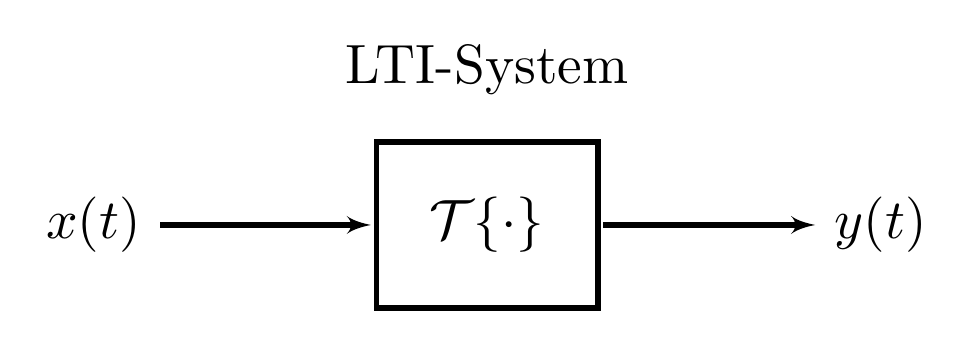
\begin{tikzpicture}[auto,>=latex', transform shape, scale=2]

\tikzstyle{block} = [draw, shape=rectangle, minimum height=3em, minimum width=4em, node distance=2cm, line width=2pt]
\tikzstyle{branch} = [fill,shape=circle,minimum size=4pt,inner sep=0pt]

\node at (-2.5,0) (input) {$x(t)$};
\node [block] (t) {$\mathcal{T\{\cdot\}}$} node[above=2em] {LTI-System};
\node at (2.5,0) (output) {$y(t)$};

\begin{scope}[line width=2pt]
     \draw[->] (input) -- (t);
     \draw[->] (t) -- (output);
\end{scope}
\end{tikzpicture}
\end{document}
